
 \section{Website}

 \subsection{Overview}
 \paragraph{}
 The website is a hosting service for uploading, downloading and managing the users files. Microsoft's ASP.NET MVC was used to create the website and Azure was used for its web hosting and file storage tools.
 
 \paragraph{}
 Users can create an account to store and share 3D models with other users. Once a user has an account, they can upload a 3D model as one of the websites supported file types. A user can download the model as any of the supported file types or generate a QR code that can be used for quick download using the mobile app or any other QR code readers.

\subsection{User Interface}
The user interface was designed to be very simple. The UI is comprised of four main pages with a navigation bar to get the pages
    \paragraph{Public Content Page}

        \begin{figure}[H]
        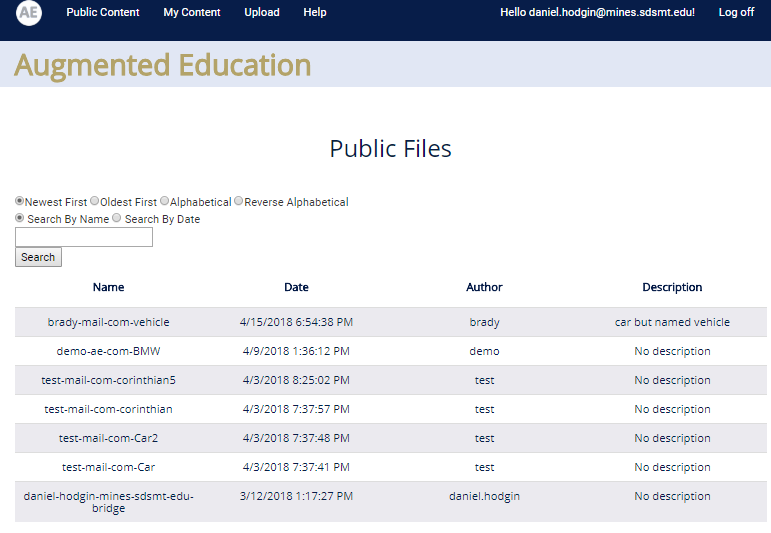
\includegraphics[width=0.5\textwidth]{Web/PublicPage}
        \centering
        \caption{Public Content Page}
        \label{fig:PublicContent}
        \end{figure}

        This is the main landing page for the website. From here users are able to browse the public files to download and generate QR code. Users do not need to be signed in or have an account to access the information on this page.

    \paragraph{My Content Page}
        \begin{figure}[H]
        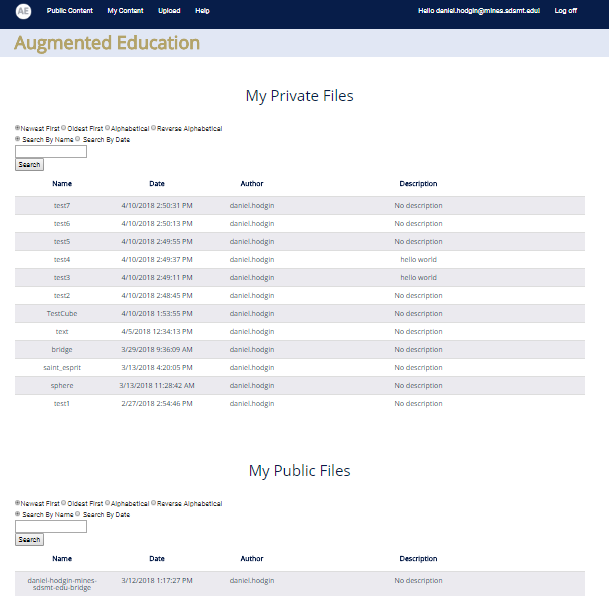
\includegraphics[width=0.5\textwidth]{Web/MyContent}
        \centering
        \caption{My Content Page}
        \label{fig:MyContent}
        \end{figure}

        This page displays all of the content that a user has uploaded. Here a user can browse their private and public files to download and generate QR codes. Users also have the ability to delete files. Users must have an account to access this page.

    \paragraph{Upload Page}
        \begin{figure}[H]
        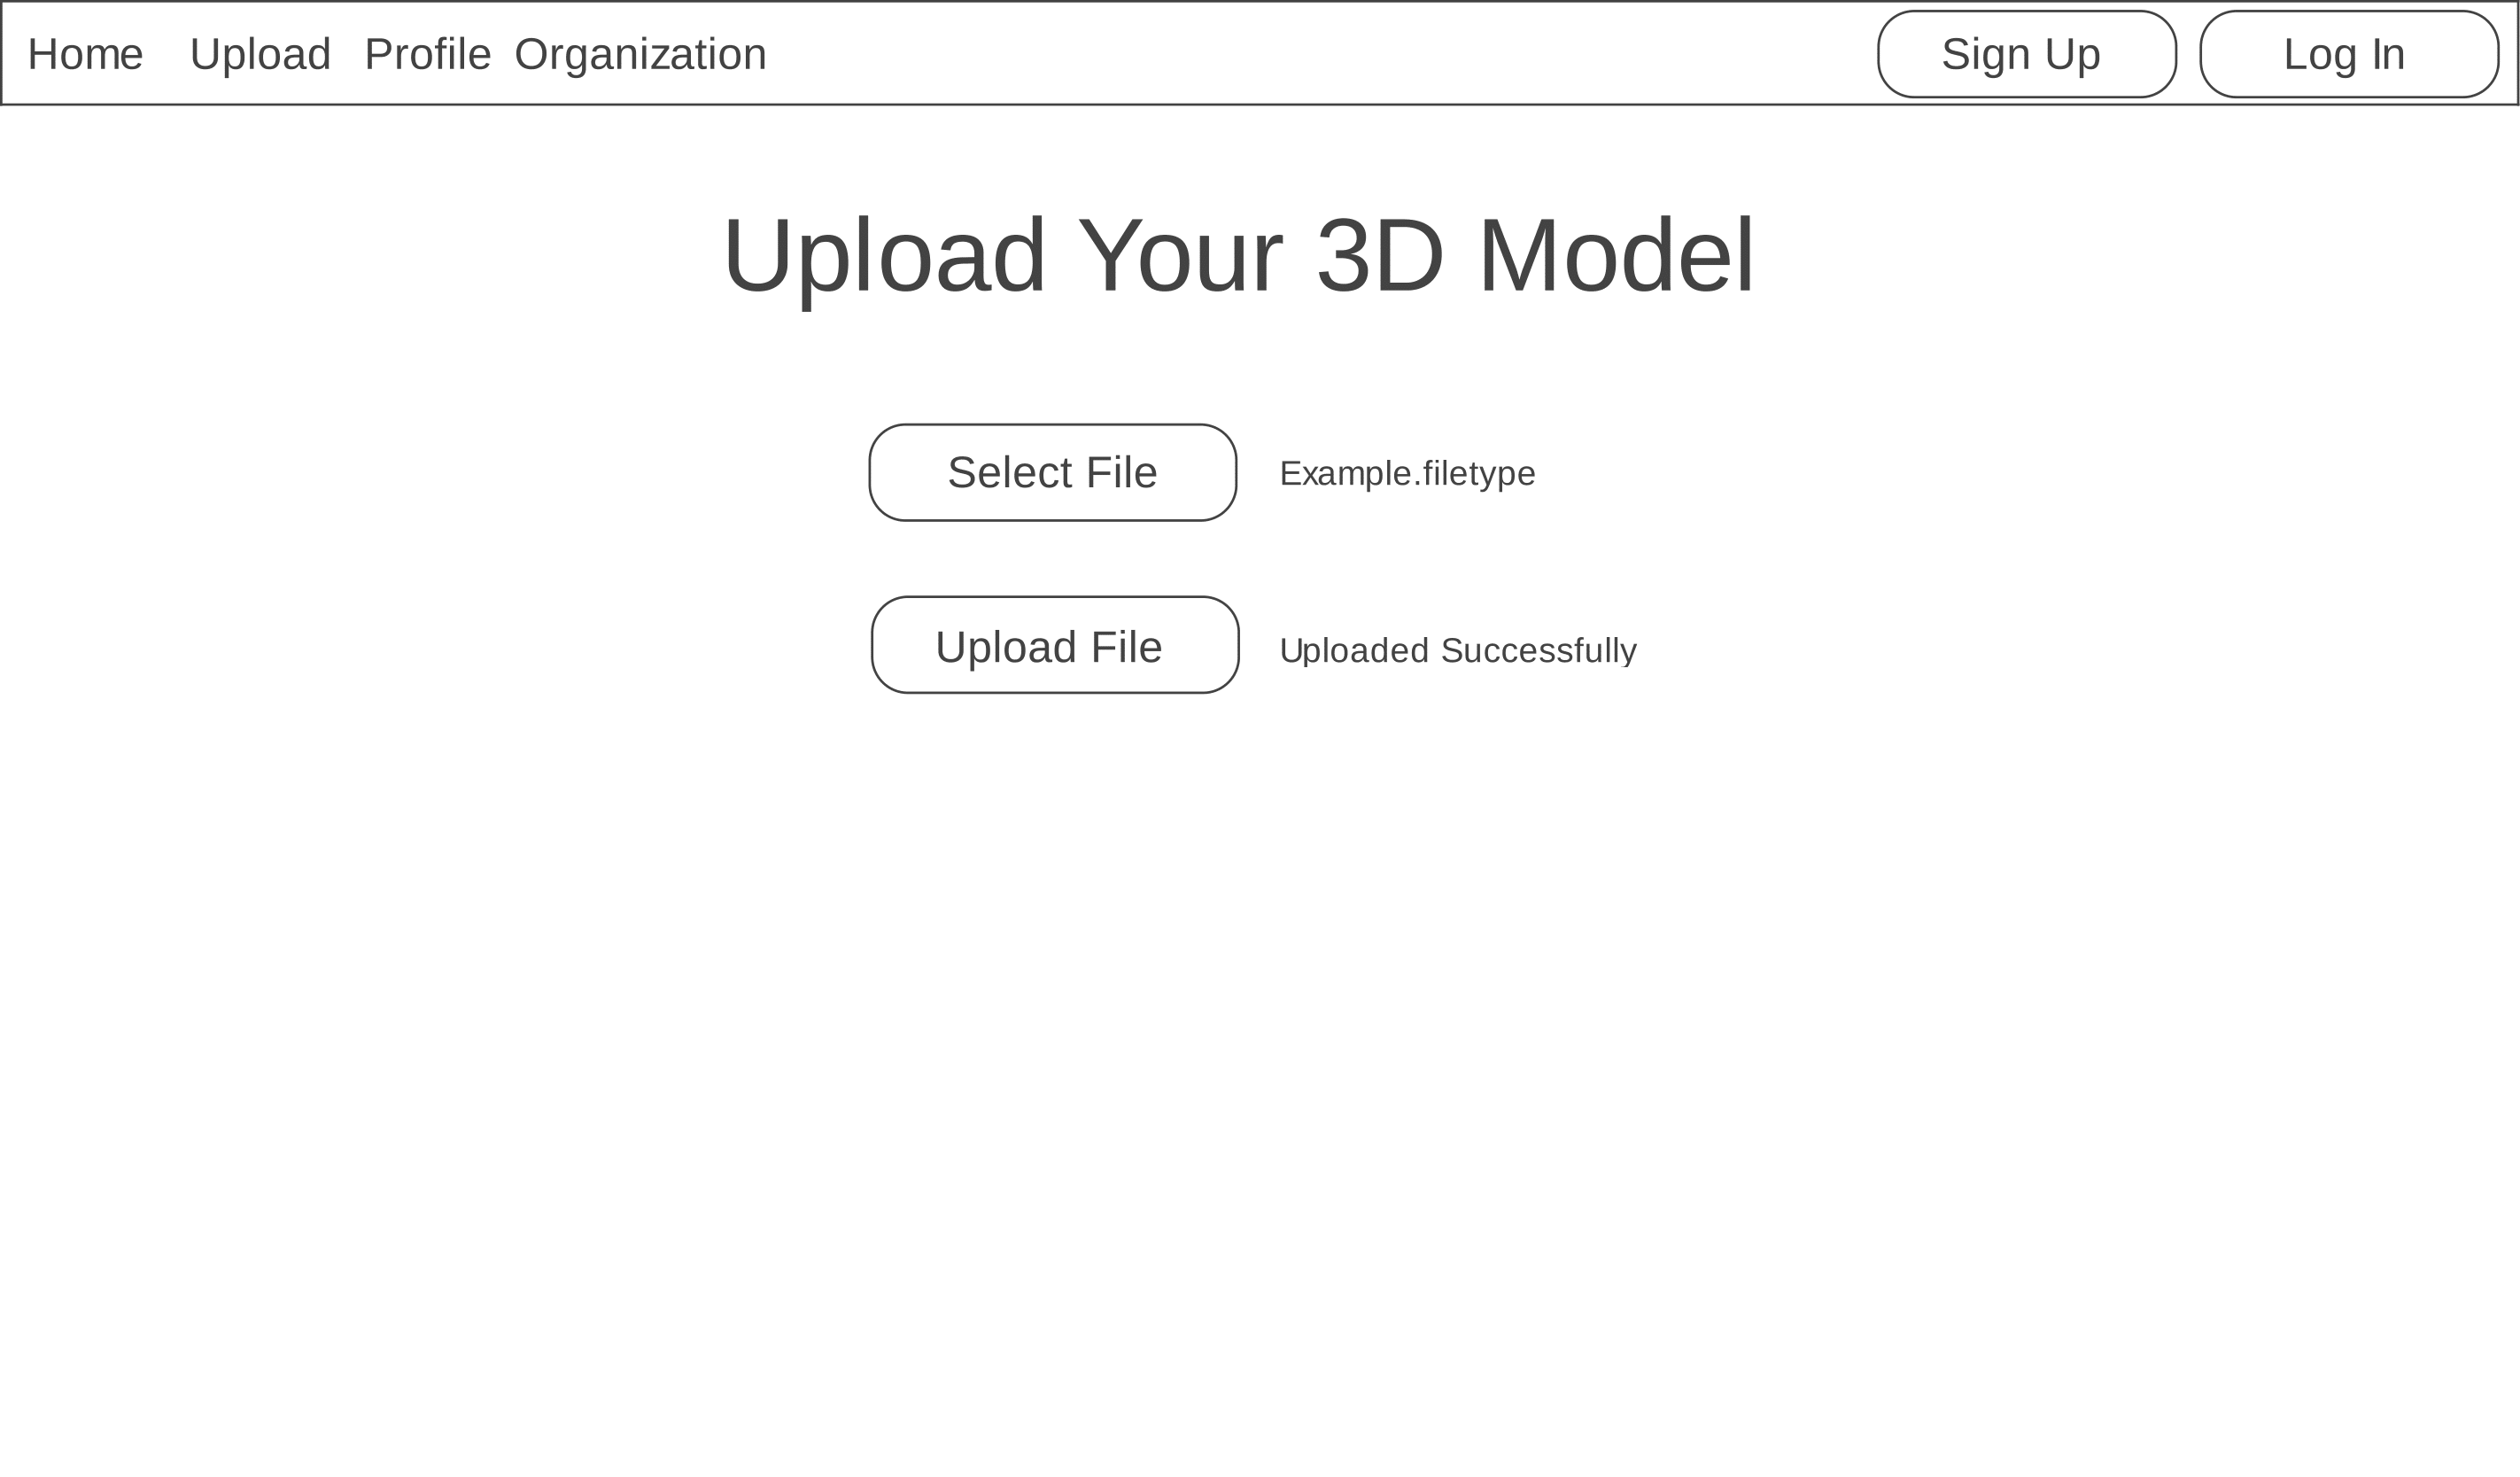
\includegraphics[width=0.5\textwidth]{Web/Upload}
        \centering
        \caption{Upload Page}
        \label{fig:UploadPage}
        \end{figure}

        This page allows users to upload 3D models. Users can upload a material file if it is an OBJ file. The user can add a description, specify an alternate name, and make the file public. Users must have an account and be signed in to access this page.

    \paragraph{Help Page}
        \begin{figure}[H]
        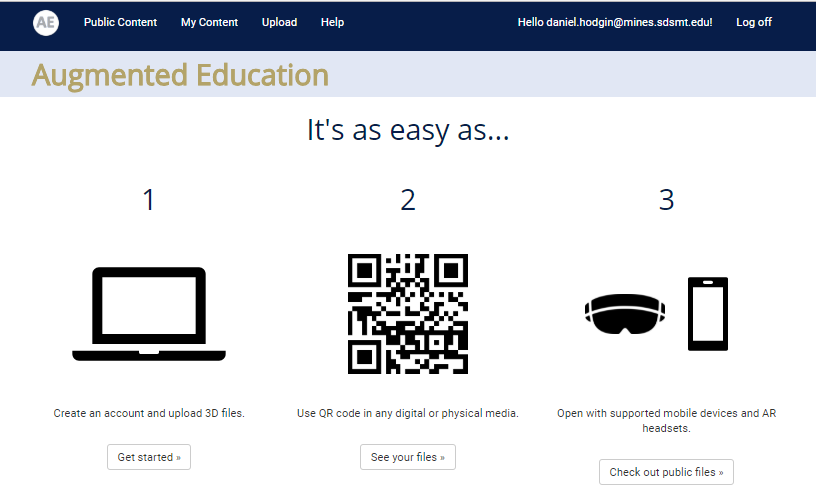
\includegraphics[width=0.5\textwidth]{Web/Help}
        \centering
        \caption{Upload Page}
        \label{fig:HelpPage}
        \end{figure}
    
        This page just gives a simple tutorial on how to uses the website.

\subsection{Technologies Used}

    As stated earlier in this document, this product is making use
    of the Microsoft environment for its tools. Below is an in-depth 
    breakdown of the tools currently being used:

    \begin{itemize}
    \item ASP.NET MVC
    \begin{itemize}
        \item An MVC web architecture, where the backend logic is written in controller classes
        that send and receive data from the client.
        \item It allows for dynamic HTML pages using a Razor syntax. Razor allows
        you to embed C\# Code into the HTML and execute logic.
    \end{itemize}
    
    \item Azure
        \begin{itemize}
            \item Microsoft cloud hosting services.
            \item Allows for simple database and web hosting.
            \item Paid features are offered free to students.
        \end{itemize}
    \end{itemize}

    These tools make up the core development of this website. The website is also
    making use of other smaller packages to handles user authentication and database management.

    The website also implements the file conversion software that is described later.
    The file conversion was written in C++, so it couldn't be compiled with the website.
    The workaround was that the file conversion was compiled into an executable that can be used through a system command to convert the file.


    \subsection{Data Flow}
    The website acts as an intermediary between the user and the cloud. Data flow for the website can be broken into a upload and download data flow.

    \paragraph{Upload Data Flow}
    \begin{itemize}
        \item Once a user upload a file it is temporarily save on the server.
        \item If the file is not a FBX file it is converted to a FBX file.
        \item The file is then uploaded to Azure blob storage for long term storage.
        \item The file on the server is then deleted on a successful upload to Azure.
    \end{itemize}

    \paragraph{Download Data Flow}
    \begin{itemize}
        \item When a user requests to download a file or generate a QR code, the file name and type is sent to the server.
        \item The server pulls the file from Azure and temporarily save it to the server.
        \item If a download is requested, it does a conversion if necessary and send the file to the user.
        \item If a QR code is generated, it does a conversion if necessary and then saves it back to Azure storage and returns a link to the file in Azure embedded in a QR code.
    \end{itemize}


\subsection{Design Details}

    \subsubsection{Overview}

    The website was written in C\# with the ASP.NET MVC framework. The main logic
    of the website are contained in two controllers
    \begin{itemize}
        \item Upload Controller
        \begin{itemize}
            \item Handles upload from client to the server.
            \item Uses File Conversion executable to convert to FBX file type
            \item Stores file on the web.
        \end{itemize}
        \item Download
        \begin{itemize}
            \item Uploads Model tag from client to server.
            \item Finds associated store model.
            \item Returns model to the client.
        \end{itemize}
    \end{itemize}

    \subsubsection{Code Structure}
    As stated before the website is using ASP.NET MVC framework. 
    The logic happens in the controllers and is split up into the upload and download controller.
    
    \paragraph{Parameter Passing}
    \hfill \break
    The main functions that are being used are the upload and download function.
    
    \begin{itemize}
        \item Upload Function
        \begin{itemize}
           \item HttpPostedFileBase - http message sent from client to server containing the file
           \item The message is parsed to retrieve the file and save to the web.
        \end{itemize}

        \item Download Function
        \begin{itemize}
            \item input string ModelTag - string containing the reference tag to the model.
            \item output httpresponse - http message sent from server to client containing the file. 
        \end{itemize}
    \end{itemize}